% =====================================================================
%  Energy-audited Lagrangian simulation and sensitivity-gradient tipping
%  for cable-only locomotion of a six-bar tensegrity rover
%
%  Build:   cd paper && latexmk -pdf main.tex
%  Numbers: every quantitative statement comes from \input{numbers.tex}
%           and \input{tables.tex}, generated by
%             npm run experiments && npm run paper:data
%           so the text can never disagree with the measured data.
%
%  TODO before submission (search for "TODO"):
%   * authors, affiliations, funding;
%   * exact citation of the non-minimal-coordinate preprint (title page
%     missing from the repository copy);
%   * entries in references.bib marked VERIFY.
% =====================================================================
\documentclass[conference]{IEEEtran}
\IEEEoverridecommandlockouts
\usepackage{amsmath,amssymb,amsfonts}
\usepackage{algorithm}
\usepackage{algpseudocode}
\usepackage{graphicx}
\usepackage{booktabs}
\usepackage{adjustbox}
\usepackage{siunitx}
\usepackage{xcolor}
\usepackage{cite}
\usepackage[hidelinks]{hyperref}

\graphicspath{{../results/paper/figures/}}
% Auto-generated by tools/make_numbers.mjs -- do not edit by hand.
\newcommand{\nSgtSpeed}{0.091}
\newcommand{\nSgtSpeedStd}{0.026}
\newcommand{\nSgtProgress}{1.81}
\newcommand{\nSgtRmse}{0.253}
\newcommand{\nSgtSuccess}{100}
\newcommand{\nSgtAid}{0}
\newcommand{\nSgtCot}{11.4}
\newcommand{\nSgtSolveMs}{0.68}
\newcommand{\nSgtSolveMax}{17.4}
\newcommand{\nSgtResidual}{1.0\times 10^{-9}}
\newcommand{\nSgtBar}{2.3\times 10^{-11}}
\newcommand{\nHeuSpeed}{0.004}
\newcommand{\nHeuSpeedStd}{0.000}
\newcommand{\nHeuProgress}{0.07}
\newcommand{\nHeuRmse}{0.083}
\newcommand{\nHeuSuccess}{0}
\newcommand{\nHeuAid}{0}
\newcommand{\nHeuCot}{142.4}
\newcommand{\nHeuSolveMs}{0.47}
\newcommand{\nHeuSolveMax}{43.1}
\newcommand{\nHeuResidual}{9.9\times 10^{-10}}
\newcommand{\nHeuBar}{3.4\times 10^{-11}}
\newcommand{\nLqrSpeed}{0.002}
\newcommand{\nLqrSpeedStd}{0.000}
\newcommand{\nLqrProgress}{0.03}
\newcommand{\nLqrRmse}{0.129}
\newcommand{\nLqrSuccess}{0}
\newcommand{\nLqrAid}{0}
\newcommand{\nLqrCot}{--}
\newcommand{\nLqrSolveMs}{0.65}
\newcommand{\nLqrSolveMax}{21.8}
\newcommand{\nLqrResidual}{1.0\times 10^{-9}}
\newcommand{\nLqrBar}{7.9\times 10^{-12}}
\newcommand{\nIlqrSpeed}{0.005}
\newcommand{\nIlqrSpeedStd}{0.000}
\newcommand{\nIlqrProgress}{0.10}
\newcommand{\nIlqrRmse}{0.081}
\newcommand{\nIlqrSuccess}{0}
\newcommand{\nIlqrAid}{0}
\newcommand{\nIlqrCot}{111.8}
\newcommand{\nIlqrSolveMs}{0.90}
\newcommand{\nIlqrSolveMax}{15.5}
\newcommand{\nIlqrResidual}{9.9\times 10^{-10}}
\newcommand{\nIlqrBar}{6.1\times 10^{-12}}
\newcommand{\nMpcSpeed}{0.004}
\newcommand{\nMpcSpeedStd}{0.000}
\newcommand{\nMpcProgress}{0.08}
\newcommand{\nMpcRmse}{0.084}
\newcommand{\nMpcSuccess}{0}
\newcommand{\nMpcAid}{0}
\newcommand{\nMpcCot}{132.0}
\newcommand{\nMpcSolveMs}{0.82}
\newcommand{\nMpcSolveMax}{12.5}
\newcommand{\nMpcResidual}{9.9\times 10^{-10}}
\newcommand{\nMpcBar}{6.1\times 10^{-12}}
\newcommand{\nLegSpeed}{0.522}
\newcommand{\nLegSpeedStd}{0.023}
\newcommand{\nLegProgress}{10.45}
\newcommand{\nLegRmse}{0.006}
\newcommand{\nLegSuccess}{100}
\newcommand{\nLegAid}{50}
\newcommand{\nLegCot}{1.1}
\newcommand{\nLegSolveMs}{0.15}
\newcommand{\nLegSolveMax}{5.2}
\newcommand{\nLegResidual}{1.1\times 10^{1}}
\newcommand{\nLegBar}{1.9\times 10^{-4}}
\newcommand{\pDaeResidual}{1.0\times 10^{-9}}
\newcommand{\pDaeBar}{2.3\times 10^{-11}}
\newcommand{\pNoERowResidual}{1.5\times 10^{1}}
\newcommand{\pLegacyResidual}{1.1\times 10^{1}}
\newcommand{\pDaeNum}{7.3\times 10^{-3}}
\newcommand{\pNoERowNum}{3.9\times 10^{1}}
\newcommand{\pLegacyNum}{6.8\times 10^{3}}
\newcommand{\pLegacyBar}{1.3\times 10^{-7}}
\newcommand{\pDaeStepDrift}{7.6\times 10^{-2}}
\newcommand{\pDaeDriftAbs}{17.0}
\newcommand{\pNoERowDriftAbs}{33.1}
\newcommand{\pLegacyDriftAbs}{11.0}
\newcommand{\pLegacyStepDrift}{1.1\times 10^{-3}}
\newcommand{\pLegacyAidShare}{50}
\newcommand{\dcDaeTwoAbs}{15.4}
\newcommand{\dcDaeTwoSigned}{-4.4}
\newcommand{\dcDaeTwoRate}{0.77}
\newcommand{\dcDaeTwoStep}{7.6\times 10^{-2}}
\newcommand{\dcDaeTwoCable}{37.7}
\newcommand{\dcDaeOneAbs}{7.6}
\newcommand{\dcDaeOneSigned}{-4.3}
\newcommand{\dcDaeOneRate}{0.38}
\newcommand{\dcDaeOneStep}{1.9\times 10^{-2}}
\newcommand{\dcDaeOneCable}{61.5}
\newcommand{\dcLegTwoAbs}{11.0}
\newcommand{\dcLegTwoSigned}{-11.0}
\newcommand{\dcLegTwoRate}{0.55}
\newcommand{\dcLegTwoStep}{1.1\times 10^{-3}}
\newcommand{\dcLegTwoCable}{7004.4}
\newcommand{\dcLegOneAbs}{5.5}
\newcommand{\dcLegOneSigned}{-5.5}
\newcommand{\dcLegOneRate}{0.28}
\newcommand{\dcLegOneStep}{2.9\times 10^{-4}}
\newcommand{\dcLegOneCable}{3729.2}
\newcommand{\aFullSpeed}{0.080}
\newcommand{\aFullSpeedStd}{0.029}
\newcommand{\aFullCot}{13.4}
\newcommand{\aFullSuccess}{100}
\newcommand{\aFullTips}{8.7}
\newcommand{\aNoPayloadSpeed}{0.076}
\newcommand{\aNoPayloadSpeedStd}{0.005}
\newcommand{\aNoPayloadCot}{7.7}
\newcommand{\aNoPayloadSuccess}{100}
\newcommand{\aNoPayloadTips}{8.7}
\newcommand{\aNoFeasSpeed}{0.102}
\newcommand{\aNoFeasSpeedStd}{0.034}
\newcommand{\aNoFeasCot}{8.9}
\newcommand{\aNoFeasSuccess}{100}
\newcommand{\aNoFeasTips}{10.3}
\newcommand{\aNoGeoSpeed}{0.056}
\newcommand{\aNoGeoSpeedStd}{0.010}
\newcommand{\aNoGeoCot}{23.5}
\newcommand{\aNoGeoSuccess}{67}
\newcommand{\aNoGeoTips}{5.7}
\newcommand{\aSparseSpeed}{0.085}
\newcommand{\aSparseSpeedStd}{0.002}
\newcommand{\aSparseCot}{5.6}
\newcommand{\aSparseSuccess}{100}
\newcommand{\aSparseTips}{9.3}
\newcommand{\aNoERowSpeed}{0.104}
\newcommand{\aNoERowSpeedStd}{0.029}
\newcommand{\aNoERowCot}{9.4}
\newcommand{\aNoERowSuccess}{100}
\newcommand{\aNoERowTips}{10.3}
\newcommand{\aLegacySpeed}{0.026}
\newcommand{\aLegacySpeedStd}{0.000}
\newcommand{\aLegacyCot}{49.1}
\newcommand{\aLegacySuccess}{0}
\newcommand{\aLegacyTips}{14.0}
\newcommand{\sNomSpeed}{0.080}
\newcommand{\sNomSpeedStd}{0.029}
\newcommand{\sNomSuccess}{100}
\newcommand{\sNomRec}{--}
\newcommand{\sImpSpeed}{0.094}
\newcommand{\sImpSpeedStd}{0.017}
\newcommand{\sImpSuccess}{100}
\newcommand{\sImpRec}{0.09}
\newcommand{\sPushSpeed}{0.085}
\newcommand{\sPushSpeedStd}{0.006}
\newcommand{\sPushSuccess}{100}
\newcommand{\sPushRec}{2.00}
\newcommand{\sGaussSpeed}{0.065}
\newcommand{\sGaussSpeedStd}{0.016}
\newcommand{\sGaussSuccess}{67}
\newcommand{\sGaussRec}{--}
\newcommand{\sLapSpeed}{0.026}
\newcommand{\sLapSpeedStd}{0.016}
\newcommand{\sLapSuccess}{0}
\newcommand{\sLapRec}{--}
\newcommand{\sOutSpeed}{0.034}
\newcommand{\sOutSpeedStd}{0.023}
\newcommand{\sOutSuccess}{33}
\newcommand{\sOutRec}{--}
\newcommand{\sStiffSpeed}{0.057}
\newcommand{\sStiffSpeedStd}{0.002}
\newcommand{\sStiffSuccess}{100}
\newcommand{\sStiffRec}{--}
\newcommand{\sFricSpeed}{0.104}
\newcommand{\sFricSpeedStd}{0.024}
\newcommand{\sFricSuccess}{100}
\newcommand{\sFricRec}{--}
\newcommand{\sMassSpeed}{0.083}
\newcommand{\sMassSpeedStd}{0.016}
\newcommand{\sMassSuccess}{100}
\newcommand{\sMassRec}{--}
\newcommand{\sDelaySpeed}{0.050}
\newcommand{\sDelaySpeedStd}{0.003}
\newcommand{\sDelaySuccess}{67}
\newcommand{\sDelayRec}{--}
\newcommand{\gFourSpeed}{0.074}
\newcommand{\gFourSpeedStd}{0.019}
\newcommand{\gFourResidual}{1.0\times 10^{-9}}
\newcommand{\gSevenSpeed}{0.087}
\newcommand{\gSevenSpeedStd}{0.020}
\newcommand{\gSevenResidual}{1.5\times 10^{-2}}
\newcommand{\baseBestProgress}{0.10}
\newcommand{\baseBestSpeed}{0.0052}
\newcommand{\speedRatio}{25}

% Auto-generated by tools/make_extension_tables.mjs -- do not edit by hand.
\newcommand{\gpsIterations}{8}
\newcommand{\gpsSamples}{114k}
\newcommand{\gpsEvalConditions}{4}
\newcommand{\gpsPolicyProgress}{1.89}
\newcommand{\gpsSgtProgress}{2.11}
\newcommand{\gpsTeacherProgress}{2.27}
\newcommand{\gpsRatio}{89}
\newcommand{\gpsTeacherRatio}{83}
\newcommand{\gpsPolicyMs}{0.73}
\newcommand{\gpsSgtMs}{0.53}
\newcommand{\gpsPolicyAborts}{0.50}
\newcommand{\gpsBestPolicy}{2.59}
\newcommand{\gpsBestSgt}{2.35}
\newcommand{\shConditions}{10}
\newcommand{\shSlackOffSgt}{35.1}
\newcommand{\shSlackOnSgt}{2.7}
\newcommand{\shSlackOffGps}{33.6}
\newcommand{\shSlackOnGps}{1.6}
\newcommand{\shAnySlackOff}{100}
\newcommand{\shTensionOffSgt}{6.2}
\newcommand{\shTensionOnSgt}{18.0}
\newcommand{\shProgOffSgt}{1.49}
\newcommand{\shProgOnSgt}{2.20}
\newcommand{\shProgGainSgt}{48}
\newcommand{\shProgBetterSgt}{8}
\newcommand{\shAbortOffSgt}{1.1}
\newcommand{\shAbortOnSgt}{0.0}
\newcommand{\shProgOffGps}{1.32}
\newcommand{\shProgOnGps}{1.29}
\newcommand{\shFilteredRuns}{20}
\newcommand{\shClearViol}{3}
\newcommand{\shClearMin}{0.008}
\newcommand{\shOuterViol}{8}
\newcommand{\shMs}{3.6}
\newcommand{\sagInitialHeight}{0.467}
\newcommand{\sagMeanHeight}{0.394}
\newcommand{\sagPercent}{16}
\newcommand{\sagDesignTension}{50}
\newcommand{\sagMeanTension}{5.7}


\newcommand{\vect}[1]{\boldsymbol{#1}}
\newcommand{\R}{\mathbb{R}}
\newcommand{\todo}[1]{\textcolor{red}{[TODO: #1]}}

\begin{document}

\title{Sensitivity-Gradient Tipping, MPC-Guided Policy Search and
Suspension Integrity for Cable-Only Locomotion of an Energy-Audited
Six-Bar Tensegrity Rover}

\author{\IEEEauthorblockN{\todo{Author names}}
\IEEEauthorblockA{\todo{Department of Robotics, Institution, City, Country}\\
\todo{email}}}

\maketitle

% ---------------------------------------------------------------------
\begin{abstract}
Simulation results for rolling tensegrity robots are hard to trust when
the simulator itself can create or destroy energy: penalty-spring bars
followed by position projection, ground clamps and ``helper'' torques
can all produce apparent locomotion that the cables alone could not.
We present a simulator and a gait for a six-bar tensegrity rover with an
internal payload in which every joule is accounted for. The shell is
modelled in non-minimal Cartesian coordinates with the consistent
rigid-bar mass matrix and exact bar-length multipliers; contact is a
passive Hunt--Crossley law whose elastic part is a potential; and a
work ledger books every force and every projection and measures, at
each step and before any correction, the energy that no booked work
explains. This per-step drift is first-order discretization error
(it halves when the time step is halved) and is then removed by a
minimum-norm constraint-and-energy corrector. The audit shows that a
conventional penalty+SHAKE engine exchanges $\pLegacyNum$\,J with its
position projection to keep the bars rigid and, in its interactive
form, takes \pLegacyAidShare\,\% of its energy input from non-physical
aids. On the audited simulator we propose Sensitivity-Gradient Tipping
(SGT), which differentiates the pinned quasi-static equilibrium,
including the softening geometric stiffness of the compressed bars, to
obtain the sensitivity of the centre of mass to all 36 shell and
payload cables, and drives it across a forward support edge within the
actuator box. With cables only, SGT reaches \nSgtSpeed\,m/s
(\nSgtSuccess\,\% success over 5 seeds), whereas reduced-order LQR, iLQR
and MPC schedulers over a support-face primitive advance at most
\baseBestProgress\,m in 20\,s under identical limits. Ablations show
that the geometric-stiffness term is the component that matters, and
stress tests expose a sensitivity to heavy-tailed sensor noise.
Building on SGT we contribute two further components. \emph{MPC + GPS}
is MPC-guided policy search with a receding-horizon QP teacher on the
same sensitivity model, which reduces exactly to SGT in a limit; the
learned, permutation-equivariant cable policy reaches \gpsRatio\,\% of
SGT's progress on held-out conditions without the per-tick KKT solve.
We further find that while rolling the shell sags by \sagPercent\,\% and
the payload cables, designed for \sagDesignTension\,N, carry only
\sagMeanTension\,N on average and are slack \shSlackOffSgt\,\% of the
time. A suspension-integrity filter that imposes discrete-time barrier
conditions on the predicted cable tensions keeps them taut
(\shSlackOnSgt\,\% slack time) in all \shConditions\ test conditions
and, by preserving the tipping shift, increases SGT's progress by
\shProgGainSgt\,\%. Code, run files and the scripts that produce every
number are released.
\end{abstract}

\begin{IEEEkeywords}
Tensegrity robots, rolling locomotion, guided policy search, control
barrier functions, energy-consistent simulation.
\end{IEEEkeywords}

% ---------------------------------------------------------------------
\section{Introduction}

Six-bar spherical tensegrities combine low mass with high impact
tolerance and have been studied as planetary landers and rovers
\cite{sabelhaus2015superball,littlefield2019kinodynamic}. They move by
\emph{punctuated rolling}: changing cable rest lengths deforms the shell
until the centre of mass (COM) leaves the triangular support face and
the structure tips onto a neighbouring face. Because hardware is
expensive and fragile, gaits are usually developed in simulation
\cite{mirletz2015reality,zhang2017deep} and transferred later.

Two practical problems limit what such simulations prove.
\emph{(i) Admissibility.} Rigid bars are often emulated by stiff
penalty springs and corrected by position projection (SHAKE/RATTLE
\cite{ryckaert1977shake,andersen1983rattle}); contacts by clamps or
restitution impulses. Each of these steps changes the mechanical energy
without a corresponding physical work term, and in interactive
simulators it is common to add ``assist'' torques or traction forces so
that a gait looks convincing. Without an audit it is impossible to tell
how much of the locomotion the cables actually produced.
\emph{(ii) Actuation.} Classic support-face gaits contract a fixed set
of cables around the current face. With a realistic actuator stroke and
a heavy internal payload, such a primitive may not move the COM far
enough to tip, regardless of how its effort is scheduled.

This paper addresses both problems.
\begin{enumerate}
\item \emph{Energy-audited simulation.} We implement the non-minimal
Cartesian Lagrangian formulation of tensegrity dynamics with the
consistent rigid-bar mass matrix, exact constraint multipliers and a
minimum-norm constraint-and-energy corrector \cite{nonminimal_preprint},
and add a passive Hunt--Crossley contact \cite{hunt1975coefficient}
whose elastic energy is part of the energy function. A \emph{work
ledger} books every force category and every projection and records
the per-step energy mismatch \emph{before} correction, which bounds any
unbooked energy source and can be checked for convergence in $\Delta t$.
\item \emph{Sensitivity-Gradient Tipping (SGT).} A cable-only gait that
linearizes the quasi-static equilibrium of shell and payload with the
support pinned, including the geometric stiffness of the compressed
bars, and commands all 36 actuators along the gradient of the COM
displacement across a forward support edge.
\item \emph{MPC + GPS (MPC-guided policy search).} A receding-horizon
QP teacher on the SGT sensitivity model with spool-rate limits and a
policy-proximity term, which reduces exactly to the SGT command in a
limit, and a permutation-equivariant per-cable policy trained from it by
guided policy search \cite{levine2013guided,zhang2016mpcgps}.
Throughout, GPS denotes Guided Policy Search.
\item \emph{Suspension integrity.} The observation that the payload
suspension of a rolling six-bar rover loses its pretension, and a
safety filter that minimally corrects any tipping controller with
discrete-time barrier conditions on the predicted cable tensions and a
shift-preserving constraint, using the sensitivities SGT already
computes.
\item \emph{Protocol and audit.} A deterministic, seed-locked benchmark
shared by the interactive application and a headless batch runner: five
baselines with identical actuator limits, impulse and step
disturbances, Gaussian/Laplace/outlier sensor noise,
stiffness/friction/mass mismatch and actuation delay, seven ablations
and three terrains (114 runs). Tables, figures and every number in the
text are generated from the run files.
\end{enumerate}
To our knowledge, the combination of a per-step energy audit with a
sensitivity-based cable-only tipping gait, a teacher for guided policy
search derived from it, and a filter for the integrity of the payload
suspension has not been reported for six-bar tensegrity rovers. All claims are restricted to simulation
(Section~\ref{sec:limits}); in particular the negative results for
the baselines concern the support-face primitive they schedule, not
the optimal-control methods as such.

% ---------------------------------------------------------------------
\section{Related Work}

\emph{Tensegrity simulation.} General engines such as MuJoCo and Bullet
\cite{todorov2012mujoco,coumans2015bullet} and dedicated tensegrity
simulators \cite{mirletz2015reality} treat bars as rigid bodies or stiff
springs; constraint drift is removed by stabilization
\cite{baumgarte1972} or projection
\cite{ryckaert1977shake,andersen1983rattle}. Structure-preserving
integrators \cite{hairer2006geometric} conserve energy for conservative
systems but do not by themselves expose energy injected by contact or
by non-physical controller aids. The class-$k$ tensegrity literature
\cite{skelton2009tensegrity} and the non-minimal Cartesian formulation
\cite{nonminimal_preprint} provide the dynamics used here.

\emph{Tensegrity locomotion.} Rolling gaits have been obtained from
hand-designed cable sequences, kinodynamic planning over gait primitives
\cite{littlefield2019kinodynamic} and reinforcement learning
\cite{zhang2017deep}. These works optimize \emph{which} primitive to
execute; SGT instead computes the primitive itself from the local
quasi-static sensitivity of the COM and is therefore complementary to
primitive-level planners.

\emph{Guided policy search.} Guided policy search trains a policy by
supervised learning on the actions of local trajectory optimizers that
are themselves kept close to the policy \cite{levine2013guided,
montgomery2016mdgps}; the MPC-guided variant uses a model-predictive
controller as teacher \cite{zhang2016mpcgps}, and PLATO executes the
policy-regularized teacher while labelling with the unregularized one
\cite{kahn2017plato}, which, like DAgger \cite{ross2011dagger}, trains
on the learner's own state distribution. Guided policy search has been
applied to SUPERball \cite{zhang2017deep}. Our teacher differs in that
it is a QP on the constrained quasi-static sensitivity of the shell
rather than on a learned or generic local model, and our learner is
shared across cables.

\emph{Safety filters.} Control barrier functions enforce forward
invariance of a safe set by a minimal correction of a nominal input
\cite{ames2017cbf}; the discrete-time condition
$h_{k+1}\ge(1-\gamma)h_k$ \cite{agrawal2017dcbf} is the form we use. We
are not aware of their use for the suspension of a tensegrity payload.

% ---------------------------------------------------------------------
\section{Energy-Audited Shell Dynamics}\label{sec:model}

\subsection{Coordinates, mass and constraints}
The shell has $n=12$ nodes $\vect q=[\vect q_1^\top\cdots\vect
q_{12}^\top]^\top\in\R^{36}$, six bars connecting node pairs $(i,j)$ and
24 outer cables; the payload core is a point mass $m_c$ suspended by 12
cables. Bar $k$ of length $l_k$, mass $m_k$ and radius $r_k$ is a
uniform cylinder, which gives the consistent $2\times2$ block mass
matrix (times $I_3$)
\begin{equation}
\vect M_k=\begin{bmatrix} a_k+m_i & b_k\\ b_k & a_k+m_j\end{bmatrix},\;
a_k=\tfrac{m_k}{4}+\tfrac{J_k}{l_k^2},\;
b_k=\tfrac{m_k}{4}-\tfrac{J_k}{l_k^2},
\end{equation}
with $J_k=\tfrac{m_k}{12}(3r_k^2+l_k^2)$ and node masses $m_i$. Because
the bars of a six-bar tensegrity are node-disjoint, $\vect M$ is block
diagonal and $\vect M^{-1}$ is available in closed form. The bar-length
constraints and their Jacobian are
\begin{equation}
R_k(\vect q)=\|\vect b_k\|^2-l_k^2=0,\quad
\vect b_k=\vect q_j-\vect q_i,\quad
\vect R_q=\partial\vect R/\partial\vect q .
\end{equation}

\subsection{Equations of motion}
With $\vect F$ collecting gravity, cable, damping, contact and payload
forces, the index-1 form of the DAE
$\vect M\ddot{\vect q}=\vect F+\vect R_q^\top\vect\lambda$ yields the
multipliers in closed form,
\begin{equation}
\vect\lambda=-\big(\vect R_q\vect M^{-1}\vect R_q^\top\big)^{-1}
\big(\vect\xi_2+\vect R_q\vect M^{-1}\vect F\big),\quad
\xi_{2,k}=2\|\dot{\vect b}_k\|^2,
\label{eq:lambda}
\end{equation}
and the bar compression $P_k=2\lambda_k l_k$. The $6\times6$ system in
\eqref{eq:lambda} is solved directly at every step
($\Delta t=2$\,ms, semi-implicit Euler).

\subsection{Constraint and energy correction}
Integration drift is removed after every step by the minimum-norm
corrector of \cite{nonminimal_preprint} (Algorithm~\ref{alg:corr}). The
residual vector stacks the position constraints, the velocity
constraints $\dot R_k=2\vect b_k^\top\dot{\vect b}_k$ and, optionally,
the energy row $E(\vect q,\dot{\vect q})-E^\star$, where $E^\star$ is
the energy predicted by the work ledger. As in \cite{nonminimal_preprint}
the scalar correction work $\delta W$ is an additional unknown, so the
minimum-norm step distributes the energy correction between the state
and an explicitly booked term instead of hiding it. Our extension is the energy
function: besides kinetic and gravitational energy it contains the
contact potential $V_c$ (below), whose gradient enters the energy row
of the Jacobian. The energy row is only enforced while
$|E-E^\star|\le\max(0.5\,\mathrm{J},0.02|E|)$, so that a gross
modelling error is reported by the ledger instead of being hidden by
the corrector. Note that with the energy row active the post-correction
residual is zero \emph{by construction}; the informative quantity is
the pre-correction drift defined below.

\begin{algorithm}[t]
\caption{Minimum-norm constraint and energy correction}\label{alg:corr}
\begin{algorithmic}[1]
\Require $\vect q,\dot{\vect q}$ after the step; ledger target $E^\star$
\State $\delta W\gets0$
\For{$it=1,\dots,10$}
  \State $\vect r\gets[\vect R;\ \dot{\vect R};\ E+V_c-(E^\star+\delta W)]$
  \If{$\|\vect r\|_\infty<\gamma$} \textbf{break} \EndIf
  \State $\vect A\gets\partial\vect r/\partial[\vect q;\dot{\vect q};\delta W]$
  \State $\vect d\gets-\vect A^\top(\vect A\vect A^\top)^{-1}\vect r$
  \Comment{minimum-norm step}
  \State $[\vect q;\dot{\vect q};\delta W]\gets[\vect q;\dot{\vect q};\delta W]+\vect d$
\EndFor
\State book $\delta W$ in the ledger (category \emph{corrector})
\end{algorithmic}
\end{algorithm}

\subsection{Passive contact}
For a node at penetration $p=\max(0,h(x,y)-z)$ into terrain $h$, the
normal force is the Hunt--Crossley law
\begin{equation}
\vect f_n=k\,p^{3/2}(1+\alpha\dot p)\,\hat{\vect n},\qquad
\hat{\vect n}\propto(-h_x,-h_y,1),
\end{equation}
whose elastic part is conservative with potential
$V_c=\tfrac{2}{5}k\,p^{5/2}$ and whose damping part is dissipative for
every $\dot p$. Tangential friction is a regularized Coulomb law
$\vect f_t=-\mu\|\vect f_n\|\,\vect v_t/\sqrt{\|\vect v_t\|^2+\epsilon^2}$,
which also only dissipates. No clamps, restitution impulses or velocity
projections are used, so the contact cannot inject energy.

\subsection{Work ledger and admissibility certificate}
The ledger stores $E=T+V_g+V_c$ and, for every force category $c$ (outer
cables, payload cables, contact, drag, disturbance, \dots), the
trapezoidal work
$W_c\mathrel{+}=\vect F_c^\top(\dot{\vect q}_k+\dot{\vect q}_{k+1})\Delta t/2$.
Position or velocity projections are booked as the energy change they
cause, and parameter changes as the jump of $E$. The certificate is
\begin{equation}
\varepsilon(t)=E(t)-E_0-\textstyle\sum_c W_c(t),
\end{equation}
evaluated after the corrector, and the per-step \emph{drift}
\begin{equation}
\delta_k=\varepsilon_k^{-}-\varepsilon_{k-1},
\end{equation}
where $\varepsilon_k^{-}$ is the residual after step $k$ but before the
energy row is applied. $\delta_k$ is the energy that step $k$ created or
destroyed without a booked cause. For a correct model it is
discretization error and must shrink with $\Delta t$; an unbooked force
or projection would not. We further report the \emph{numerical work}
$|W_{\mathrm{num}}|$ (energy changed by constraint projections and by
the corrector's $\delta W$) and the \emph{aid share}, the fraction of
the energy input supplied by non-physical categories (assist torques,
virtual forces). We call a run \emph{admissible} if the aid share is
zero, $\max_k|\delta_k|$ and $|W_{\mathrm{num}}|$ are small compared
with the actuator work, and $\delta$ converges with $\Delta t$.

% ---------------------------------------------------------------------
\section{Sensitivity-Gradient Tipping}\label{sec:sgt}

\subsection{Quasi-static sensitivity}
Between tips, the rover rests on a support face $\mathcal F$ of three
nodes that stick to the ground. Augment $\vect q$ with the core position
($n'=13$ nodes) and linearize the static equilibrium with respect to
the cable rest-length offsets $\vect u\in\R^{36}$ ($u>0$ shortens):
\begin{equation}
\begin{bmatrix}\vect K & \vect A^\top\\ \vect A & \vect 0\end{bmatrix}
\begin{bmatrix}\delta\vect q\\ \delta\vect\mu\end{bmatrix}
=\begin{bmatrix}\vect B\\ \vect 0\end{bmatrix}\delta\vect u,
\quad
\vect A=\begin{bmatrix}\vect R_q\\ \vect E_{\mathcal F}\end{bmatrix},
\label{eq:kkt}
\end{equation}
where $\vect E_{\mathcal F}$ pins the support nodes and $\vect B$
contains $\pm k\,\vect e$ for every taut cable. The tangent stiffness
assembles, for a taut cable with axial stiffness $k$, tension $t$, length
$L$ and direction $\vect e$, the element
$k\vect e\vect e^\top+\tfrac{t}{L}(\vect I-\vect e\vect e^\top)$ and,
for a bar under compression $P$, the \emph{negative} geometric stiffness
$-\tfrac{P}{L}(\vect I-\vect e\vect e^\top)$; axial bar rigidity is
already a constraint. A small relative Tikhonov term keeps the KKT
matrix regular. One LU factorization of \eqref{eq:kkt} gives all 36
columns of the COM sensitivity
$\vect S=\partial\vect c/\partial\vect u
=\tfrac{1}{m_{\mathrm{tot}}}\sum_i m_i\,\partial\vect q_i/\partial\vect u$.

\subsection{Edge selection and command}
For each edge $e$ of $\mathcal F$ with outward horizontal normal
$\vect n_e$ and midpoint $\vect p_e$, the tipping margin is
$m_e=-(\vect c-\vect p_e)^\top\vect n_e$ and the gradient of the COM
shift across the edge is $\vect g_e=\vect S_{xy}^\top\vect n_e$. Under
box limits $u_k\in[\underline u_k,\bar u_k]$ the achievable shift is
$s_e=\sum_k\max(g_{e,k}\bar u_k,\,g_{e,k}\underline u_k)$. Among edges
whose normal is aligned with the travel direction
($\vect n_e^\top\vect d\ge0.25$), SGT locks for the whole cycle the edge
with the largest reachable margin $s_e-m_e$ and commands
\begin{equation}
u_k=\bar u_k\,\mathrm{clip}\!\big(g_{e,k}/\|\vect g_e\|_\infty,\,
-\rho,\,1\big),
\end{equation}
separately normalized for shell and payload cables; $\rho$ limits cable
lengthening. A four-state machine (\textsc{Settle}$\to$\textsc{Shift}$\to$%
\textsc{Tip}$\to$\textsc{Release}) re-plans at 20\,Hz until the support
face changes, releases all cables and waits for the shell to settle
(with a timeout) before the next cycle. SGT uses only cable rest
lengths; the simulator runs with all assists disabled.

\emph{Design rationale.} A support-face primitive contracts a fixed
cable set; most of its effect is absorbed by elastic deformation that
does not move the COM over an edge. The sensitivity of the
\emph{constrained} system instead tells which cables move the COM in
the required direction, and the compressed bars soften the structure
precisely in the bending directions that tipping needs. The ablations in
Section~\ref{sec:results} test which of these ingredients matter.

% ---------------------------------------------------------------------
\section{MPC + GPS: MPC-Guided Policy Search}\label{sec:gps}

\subsection{Teacher: receding-horizon QP on the sensitivity model}
For the locked edge $e$, let
$\hat{\vect g}=[\vect g_{e,\mathrm{shell}}/\|\vect g_{e,\mathrm{shell}}\|_\infty;\
\vect g_{e,\mathrm{core}}/\|\vect g_{e,\mathrm{core}}\|_\infty]$ be the
normalized COM-shift gradient and $\tilde{\vect u}=\vect u/\bar{\vect u}$
the normalized command. Over $N$ steps of $\Delta t$ the teacher solves
\begin{equation}
\begin{aligned}
\min_{\tilde{\vect u}_{1:N}}\;&\textstyle\sum_{k=1}^{N}\big(-\hat{\vect g}^\top\tilde{\vect u}_k
+\tfrac r2\|\tilde{\vect u}_k\|^2\big)
+\tfrac{r_\Delta}{2}\textstyle\sum_{k=1}^{N}\|\tilde{\vect u}_k-\tilde{\vect u}_{k-1}\|^2\\
&+\tfrac{\lambda}{2}\|\tilde{\vect u}_1-\pi_\theta(\vect o)\|^2\\
\text{s.t.}\;&\underline{\tilde u}\le\tilde{\vect u}_k\le1,\quad
|\tilde{\vect u}_k-\tilde{\vect u}_{k-1}|\le\rho_s,
\end{aligned}
\label{eq:teacher}
\end{equation}
with $\tilde{\vect u}_0$ the current spool state and $\rho_s$ the spool
speed times $\Delta t$. The problem is separable per actuator and is
solved by projected gradient; the first step is applied and the
problem is re-solved at 20\,Hz.

\emph{Relation to SGT.} For $N=1$, $r=1$, $r_\Delta=\lambda=0$ and an
inactive rate bound, each actuator minimizes $-\hat g_k\tilde u_k+\tfrac12\tilde u_k^2$
on $[\underline{\tilde u}_k,1]$, whose solution is
$\mathrm{clip}(\hat g_k,\underline{\tilde u}_k,1)$, i.e.\ exactly the SGT
command of Section~\ref{sec:sgt}. The teacher therefore generalizes SGT
with a horizon, spool-rate limits and a smoothness term ($N=6$,
$\Delta t=50$\,ms, $r_\Delta=0.2$), and $\lambda>0$ adds the
policy-proximity term of guided policy search, the quadratic form of
the KL constraint between fixed-covariance Gaussian policies.

\subsection{Learner: a permutation-equivariant cable policy}
The policy $\pi_\theta$ does not use the KKT model. Each outer cable is
described by 20 local features in the frame of the travel direction:
midpoint relative to the COM, end-node clearances, signed distance to
the locked edge and along it, membership of its end nodes in the
support face and edge, orientation invariants
$(\vect e^\top\vect n_e)e_z$, $(\vect e^\top\vect n_e)^2$, $e_z^2$
(invariant to the sign of $\vect e$), current offset and strain, and
global context (COM velocity, gait state, margin, time in state). The
12 payload cables have 19 analogous features. One MLP with two hidden
layers of 48 units is shared by all outer cables and one of 36 units by
all payload cables, so the policy is equivariant to the cable
numbering and independent of which face the rover rests on.

\subsection{Training}
Algorithm~\ref{alg:gps} alternates a C-step, which rolls out the
teacher regularized toward the current policy plus two episodes that
execute the policy itself, and an S-step, which retrains the policy by
regression on the aggregated data. Every visited state is labelled with
the \emph{unregularized} teacher, as in PLATO \cite{kahn2017plato}. We
use $\lambda_i\in\{0,0.5,1,2,\dots\}$, four 15\,s episodes per
iteration over Levels 1 and 3 and goals straight ahead or offset by
$\pm8$ to $\pm10$\,m, and \gpsIterations\ iterations
(\gpsSamples\ labelled actuator samples).

\begin{algorithm}[t]
\caption{MPC-guided policy search (MPC + GPS)}\label{alg:gps}
\begin{algorithmic}[1]
\State $\mathcal D\gets\emptyset$; roll out teacher \eqref{eq:teacher} with $\lambda=0$; add $(\vect o,\tilde{\vect u}^\star)$ to $\mathcal D$
\For{$i=1,\dots,I$}
  \State fit $\pi_\theta$ on $\mathcal D$ (Adam, mean-squared error)
  \State roll out teacher with $\lambda_i$ \Comment{C-step, executes $\tilde{\vect u}_\lambda$}
  \State roll out $\pi_\theta$ \Comment{learner's own states}
  \State label every state with teacher $\lambda=0$; add to $\mathcal D$
\EndFor
\end{algorithmic}
\end{algorithm}

\subsection{Deployment}
At run time the policy replaces the per-tick KKT solve while the
\textsc{Settle}--\textsc{Release} state machine is kept. Choosing the
edge by alignment alone sent the policy to edges it could not tip over;
the deployed controller therefore solves \eqref{eq:kkt} once per tip
cycle to pick the edge with the largest reachable margin, as the
teacher does, and excludes edges that aborted from the same face.

% ---------------------------------------------------------------------
\section{Suspension-Integrity Filter}\label{sec:shield}

\subsection{Observation}
Gravity and the outer-cable actuation compress the shell while it
rolls: under SGT the mean node height drops from \sagInitialHeight\,m to
\sagMeanHeight\,m (\sagPercent\,\%). The node-to-payload distances
shrink with it, and the payload cables, pretensioned to
\sagDesignTension\,N, carry \sagMeanTension\,N on average; at least one
of the 12 is slack in \shAnySlackOff\,\% of the samples
(Table~\ref{tab:shield}). The ``suspended'' payload is therefore loose in
the cage for most of the motion.

\subsection{Filter}
Let $\vect u_{\mathrm{nom}}\in\R^{36}$ be the command of any tipping
controller (SGT, the teacher or the policy). The filter returns
\begin{equation}
\begin{aligned}
\vect u^\star=\arg\min_{\vect u}\;&\tfrac12(\vect u-\vect u_{\mathrm{nom}})^\top\vect W(\vect u-\vect u_{\mathrm{nom}})\\
\text{s.t.}\;&\hat h_c(\vect u)\ge(1-\gamma)\,h_c,\quad c\in\mathcal C,\\
&\hat{\vect g}^\top(\vect u-\vect u_0)\ge\hat{\vect g}^\top(\vect u_{\mathrm{nom}}-\vect u_0),\\
&\underline{\vect u}\le\vect u\le\bar{\vect u},
\end{aligned}
\label{eq:shield}
\end{equation}
where $\vect u_0$ is the current command and $\hat h_c$ is the first-order
prediction of a safety function from the displacement sensitivities
$\vect X=\partial\vect q/\partial\vect u$ that \eqref{eq:kkt} already
provides. For a cable between nodes $i,j$ with stiffness $k$, rest
length $l_0$ and direction $\vect e$,
$\hat T(\vect u)=k\big(L-l_0+u_{\mathrm{self}}+\vect e^\top(\vect X_j-\vect X_i)(\vect u-\vect u_0)\big)$.
The safety set $\mathcal C$ contains payload-cable tension
$T\ge10$\,N, outer-cable tension $T\le150$\,N and payload-to-rod
clearance $d\ge0.08$\,m (core radius 0.05\,m), the latter linearized at
the closest point of each rod. The barrier condition is the
discrete-time form of \cite{agrawal2017dcbf}: it keeps a satisfied
constraint satisfied and restores a violated one at rate $\gamma=0.3$
per control step. The second constraint preserves the nominal
command's predicted COM shift across the locked edge; without it the
filter cancels the payload-cable slackening that SGT uses to tip and
costs progress; with it the filter must re-route the tipping effort,
mainly by pulling the leading payload cables. It is dropped if it
conflicts with the barriers. $\vect W$ weights outer cables ten times
more than payload cables, so corrections are made mainly with the
payload suspension. The QP is solved by accelerated projected gradient
on the dual \cite{beck2009fista} with the box kept exact in the primal.

\emph{Scope of the guarantee.} The conditions hold for the quasi-static
prediction $\hat h$. Tumbling and impacts are inertial events that this
prediction does not contain; the closed-loop results below are
therefore empirical, and we report where they fail.

% ---------------------------------------------------------------------
\section{Experimental Protocol}\label{sec:setup}

\emph{Platform.} Shell radius 0.5\,m (bar length 0.851\,m), 12 nodes of
0.2\,kg, six bars of 0.3\,kg, payload 1.6\,kg (5.8\,kg in total);
cable stiffness 1200\,N/m (payload cables 1600\,N/m). Every cable-only
method uses the same actuator box: stroke 0.15\,m (30\,\% of the
0.49\,m rest length) for shell and payload cables and 0.20\,m/s spool
speed. Physics runs at 500\,Hz, controllers at 20\,Hz. Unless stated
otherwise all runs use the DAE core with Algorithm~\ref{alg:corr},
passive contact and zero aids, on terrain Level~1 for 20\,s.

\emph{Methods.} \emph{SGT} (proposed). \emph{Support-face heuristic}:
the fixed contraction primitive around the current face. \emph{LQR,
iLQR, QP-MPC}: the controllers of the original code base, which solve a
two-state reduced-order rolling model (speed along the goal, height
deviation) for a normalized effort $u\in[-1,1]$ that scales the same
support-face primitive---Riccati backward pass, nonlinear iLQR with line
search, and box-constrained projected-gradient MPC, respectively.
\emph{Legacy+assist}$^\dagger$: the original penalty+SHAKE engine with
roll couple, traction, grip and corridor aids; reported as a reference
only, because it is not admissible.

\emph{MPC + GPS and filter studies.} The policy is evaluated on
\gpsEvalConditions\ held-out conditions (unseen seeds, Levels 1 and 3,
straight and $\pm6$\,m offset goals, 20\,s) against SGT and the
unregularized teacher. The filter is evaluated for SGT and the policy,
each with and without it, in \shConditions\ paired conditions (three
seeds on Level~1, two on Level~3, push, impulse, payload $+30\,\%$,
100\,ms delay, cable stiffness $-20\,\%$; 20\,s), with payload-cable
slack time, mean payload-cable tension, payload rattle (RMS of the
payload position relative to the shell centroid), 99th-percentile
payload acceleration, minimal payload--rod clearance and maximal
outer-cable tension measured after the first second.

\emph{Scenarios.} Lateral impulse $\Delta v=0.5$\,m/s at $t=6$\,s; step
push 10\,N for 2\,s; Gaussian, Laplace and outlier (2\,\%, $10\times$)
noise on the measured state; cable stiffness $-20\,\%$, friction
$-40\,\%$, payload mass $+30\,\%$; actuation delay 100\,ms.

\emph{Metrics.} Mean forward speed $\bar v$; the
cross-track error $e(t)=x_c(t)-x_c(0)$ against the straight reference
heading, reported as RMS and maximum $|e|$; success ($\Delta y\ge1$\,m in 20\,s); recovery time after a
disturbance; control effort $\int\vect u^\top\vect u\,dt$; actuator
work and cost of transport
$\mathrm{CoT}=W_{\mathrm{act}}/(m g\,\Delta y)$; controller wall time
(mean and worst); $\max|\varepsilon|$, $\max_k|\delta_k|$,
$\sum_k|\delta_k|$, $|W_{\mathrm{num}}|$, maximal bar-length error and
aid share. Statistics are mean\,$\pm$\,std over seeds 1--5 (nominal) or
1--3 (other groups). A seed selects the procedural terrain outside a
flat 1.5\,m launch pad and the sensor-noise stream; methods that never
leave the pad therefore produce identical runs (zero spread).

% ---------------------------------------------------------------------
\section{Results}\label{sec:results}

% requires \usepackage{booktabs,adjustbox}
\begin{table*}[t]
\centering
\caption{Nominal cable-only locomotion on Level 1 (20\,s, 5 seeds, mean\,$\pm$\,std). All methods use the Lagrangian DAE core, passive contact and identical actuator limits.}
\label{tab:nominal}
\setlength{\tabcolsep}{2.5pt}
\footnotesize
\begin{adjustbox}{max width=\textwidth}
\begin{tabular}{lcccccccc}
\toprule
Method & $\bar v$ (m/s)\,$\uparrow$ & RMSE (m)\,$\downarrow$ & max $|e|$ (m)\,$\downarrow$ & $\int\!u^{\top}u\,dt$\,$\downarrow$ & CoT\,$\downarrow$ & $t_{\mathrm{solve}}$ (ms)\,$\downarrow$ & Succ.\ (\%)\,$\uparrow$ & Aid (\%)\,$\downarrow$ \\
\midrule
SGT (proposed) & \textbf{0.091\,$\pm$\,0.026} & 0.253\,$\pm$\,0.029 & 0.473\,$\pm$\,0.000 & \textbf{0.334\,$\pm$\,0.170} & \textbf{11.4\,$\pm$\,6.6} & 0.68\,$\pm$\,0.10 & \textbf{100} & 0 \\
Heuristic & 0.004 & 0.083 & 0.160 & 2.059 & 142.4 & \textbf{0.47\,$\pm$\,0.25} & 0 & 0 \\
LQR & 0.002 & 0.129 & 0.163 & 2.529 & -- & 0.65\,$\pm$\,0.06 & 0 & 0 \\
iLQR & 0.005 & 0.081 & 0.168 & 1.757\,$\pm$\,0.000 & 111.8 & 0.90\,$\pm$\,0.41 & 0 & 0 \\
QP-MPC & 0.004 & 0.084 & 0.175 & 1.859\,$\pm$\,0.000 & 132.0 & 0.82\,$\pm$\,0.05 & 0 & 0 \\
Legacy+assist$^\dagger$ & 0.522\,$\pm$\,0.023 & 0.006\,$\pm$\,0.002 & 0.017\,$\pm$\,0.006 & 0.636\,$\pm$\,0.060 & 1.1\,$\pm$\,0.1 & 0.15\,$\pm$\,0.02 & 100 & 50 \\
\bottomrule
\end{tabular}
\end{adjustbox}
\\[2pt]\parbox{\textwidth}{\scriptsize $^\dagger$Legacy engine with external roll couple, traction, grip and corridor aids; not physically admissible and excluded from the bold ``best'' marks. Success: $\Delta y \ge 1$\,m in 20\,s. Aid: share of the energy input supplied by non-physical aids. Cross-track errors are not marked because they are only comparable between methods that travel a similar distance.}
\end{table*}

% requires \usepackage{booktabs,adjustbox}
\begin{table*}[t]
\centering
\caption{Physical consistency of the simulator under the SGT gait (Level 1, 20\,s). $\varepsilon = E-E_0-\sum W$ is the energy no booked work explains \emph{after} correction (enforced by the energy row); $\delta_k$ is the same quantity for step $k$ \emph{before} correction, i.e.\ the per-step bound on any unbooked energy source; $|W_{\mathrm{num}}|$ is the energy changed by constraint projections and by the corrector (booked, but numerical). SGT on Level 1, 20\,s; $^\dagger$the original engine with its locomotion aids and support-face gait, for reference.}
\label{tab:physics}
\setlength{\tabcolsep}{2.5pt}
\footnotesize
\begin{adjustbox}{max width=\textwidth}
\begin{tabular}{lccccccc}
\toprule
Method & max $|\varepsilon|$ (J) & max $|\delta_k|$ (J)\,$\downarrow$ & $\sum|\delta_k|$ (J) & bar err.\ (m)\,$\downarrow$ & $|W_{\mathrm{num}}|$ (J)\,$\downarrow$ & $\bar v$ (m/s) & Aid (\%) \\
\midrule
DAE + Alg.~1, energy row & $1.0{\times}10^{-9}$ & $7.6{\times}10^{-2}$ & $1.7{\times}10^{1}$ & \textbf{$2.3{\times}10^{-11}$} & \textbf{$7.3{\times}10^{-3}$} & 0.091\,$\pm$\,0.026 & 0 \\
DAE + Alg.~1, constr.\ only & $1.5{\times}10^{1}$ & $7.1{\times}10^{0}$ & $3.3{\times}10^{1}$ & $5.9{\times}10^{-11}$ & $3.9{\times}10^{1}$ & 0.104\,$\pm$\,0.029 & 0 \\
Penalty + SHAKE (legacy) & $1.1{\times}10^{1}$ & $1.1{\times}10^{-3}$ & $1.1{\times}10^{1}$ & $1.3{\times}10^{-7}$ & $6.8{\times}10^{3}$ & 0.026 & 0 \\
Legacy + assists$^\dagger$ & $1.1{\times}10^{1}$ & $1.2{\times}10^{-3}$ & $1.1{\times}10^{1}$ & $1.9{\times}10^{-4}$ & $1.5{\times}10^{4}$ & 0.522\,$\pm$\,0.023 & 50 \\
\bottomrule
\end{tabular}
\end{adjustbox}
\end{table*}

% requires \usepackage{booktabs,adjustbox}
\begin{table}[t]
\centering
\caption{Robustness: disturbances, sensor noise, plant mismatch and actuator delay (Level 1, 20\,s, 3 seeds).}
\label{tab:stress}
\setlength{\tabcolsep}{2.5pt}
\footnotesize
\begin{adjustbox}{max width=\columnwidth}
\begin{tabular}{lccccc}
\toprule
Scenario & SGT $\bar v$ (m/s) & Heur.\ $\bar v$ (m/s) & SGT RMSE (m) & $t_{\mathrm{rec}}$ (s) & SGT succ.\ (\%) \\
\midrule
Nominal & 0.080\,$\pm$\,0.029 & 0.004 & 0.258\,$\pm$\,0.040 & -- & 100 \\
Lateral impulse 0.5 m/s & 0.094\,$\pm$\,0.017 & 0.004 & 0.266\,$\pm$\,0.011 & 0.09 & 100 \\
Step push 10 N, 2 s & 0.085\,$\pm$\,0.006 & -0.001 & 0.308\,$\pm$\,0.035 & 2.00 & 100 \\
Gaussian sensor noise & 0.065\,$\pm$\,0.016 & 0.001\,$\pm$\,0.002 & 0.219\,$\pm$\,0.030 & -- & 67 \\
Laplace sensor noise & 0.026\,$\pm$\,0.016 & -0.001\,$\pm$\,0.004 & 0.158\,$\pm$\,0.036 & -- & 0 \\
Sensor outliers (2 \%, 10x) & 0.034\,$\pm$\,0.023 & 0.002\,$\pm$\,0.002 & 0.167\,$\pm$\,0.052 & -- & 33 \\
Cable stiffness -20 \% & 0.057\,$\pm$\,0.002 & 0.002 & 0.226\,$\pm$\,0.004 & -- & 100 \\
Friction -40 \% & 0.104\,$\pm$\,0.024 & 0.002 & 0.224\,$\pm$\,0.051 & -- & 100 \\
Payload mass +30 \% & 0.083\,$\pm$\,0.016 & 0.002 & 0.249\,$\pm$\,0.022 & -- & 100 \\
Actuator delay 100 ms & 0.050\,$\pm$\,0.003 & 0.004 & 0.192\,$\pm$\,0.002 & -- & 67 \\
\bottomrule
\end{tabular}
\end{adjustbox}
\end{table}

% requires \usepackage{booktabs,adjustbox}
\begin{table}[t]
\centering
\caption{Ablation of the SGT gait and of the physics core (Level 1, 20\,s, 3 seeds).}
\label{tab:ablation}
\setlength{\tabcolsep}{2.5pt}
\footnotesize
\begin{adjustbox}{max width=\columnwidth}
\begin{tabular}{lccccc}
\toprule
Variant & $\bar v$ (m/s)\,$\uparrow$ & tips\,$\uparrow$ & RMSE (m)\,$\downarrow$ & CoT\,$\downarrow$ & Succ.\ (\%) \\
\midrule
SGT (full) & 0.080\,$\pm$\,0.029 & 8.7\,$\pm$\,3.5 & 0.258\,$\pm$\,0.040 & 13.4\,$\pm$\,8.4 & \textbf{100} \\
w/o payload actuation & 0.076\,$\pm$\,0.005 & 8.7\,$\pm$\,0.6 & 0.242\,$\pm$\,0.006 & 7.7\,$\pm$\,0.0 & \textbf{100} \\
w/o feasibility edge choice & 0.102\,$\pm$\,0.034 & 10.3\,$\pm$\,0.6 & 0.260\,$\pm$\,0.041 & 8.9\,$\pm$\,3.8 & \textbf{100} \\
w/o bar geometric stiffness & 0.056\,$\pm$\,0.010 & 5.7\,$\pm$\,1.2 & 0.194\,$\pm$\,0.001 & 23.5\,$\pm$\,4.3 & 67 \\
sparse: 8 cables & 0.085\,$\pm$\,0.002 & 9.3\,$\pm$\,0.6 & 0.286\,$\pm$\,0.025 & \textbf{5.6\,$\pm$\,0.6} & \textbf{100} \\
DAE w/o energy row & \textbf{0.104\,$\pm$\,0.029} & 10.3\,$\pm$\,2.1 & 0.242\,$\pm$\,0.026 & 9.4\,$\pm$\,5.1 & \textbf{100} \\
legacy SHAKE core & 0.026 & \textbf{14.0} & \textbf{0.043} & 49.1 & 0 \\
\bottomrule
\end{tabular}
\end{adjustbox}
\end{table}

% requires \usepackage{booktabs,adjustbox}
\begin{table}[t]
\centering
\caption{Terrain generalization (3 seeds per cell).}
\label{tab:terrain}
\setlength{\tabcolsep}{2.5pt}
\footnotesize
\begin{adjustbox}{max width=\columnwidth}
\begin{tabular}{lcccc}
\toprule
Terrain / method & $\bar v$ (m/s) & RMSE (m)\,$\downarrow$ & Succ.\ (\%) & max $|\varepsilon|$ (J) \\
\midrule
Level 1: SGT & 0.080\,$\pm$\,0.029 & 0.258\,$\pm$\,0.040 & 100 & $1.0{\times}10^{-9}$ \\
Level 1: Heuristic & 0.004 & 0.083 & 0 & $9.9{\times}10^{-10}$ \\
Level 4: SGT & 0.074\,$\pm$\,0.019 & 0.275\,$\pm$\,0.044 & 100 & $1.0{\times}10^{-9}$ \\
Level 4: Heuristic & 0.004 & 0.083 & 0 & $9.9{\times}10^{-10}$ \\
Level 7: SGT & 0.087\,$\pm$\,0.020 & 0.229\,$\pm$\,0.008 & 100 & $1.5{\times}10^{-2}$ \\
Level 7: Heuristic & 0.004 & 0.083 & 0 & $9.9{\times}10^{-10}$ \\
\bottomrule
\end{tabular}
\end{adjustbox}
\end{table}


\subsection{Physical consistency}
Table~\ref{tab:physics} compares the cores
under the same SGT command sequence. Three observations stand out.
\emph{(i) Rigidity.} The DAE core keeps the bar lengths at
$\pDaeBar$\,m; the penalty+SHAKE core reaches $\pLegacyBar$\,m and, with
the interactive aids, $\nLegBar$\,m.
\emph{(ii) Hidden energy exchange.} To keep the bars rigid, the
penalty+SHAKE core removes $\pLegacyNum$\,J by position projection
while its cables do a comparable amount of work, i.e.\ the cables
mostly pump energy into the penalty bars that the projection then
discards. The DAE core changes only $\pDaeNum$\,J numerically. With the
original locomotion aids, \pLegacyAidShare\,\% of the energy input comes
from non-physical forces, which explains its high speed
(\nLegSpeed\,m/s) in Table~\ref{tab:nominal}.
\emph{(iii) Drift.} Before correction, both cores show a per-step energy
mismatch that is first-order discretization error: for seed~1, halving
$\Delta t$ from 2 to 1\,ms reduces the accumulated $\sum_k|\delta_k|$
from \dcDaeTwoAbs\ to \dcDaeOneAbs\,J for the DAE core and from
\dcLegTwoAbs\ to \dcLegOneAbs\,J for penalty+SHAKE, and the largest
single-step mismatch of the DAE core (at the initial landing) from
$\dcDaeTwoStep$ to $\dcDaeOneStep$\,J. The energy row removes this
drift every step, so $\varepsilon$ stays at the solver tolerance
($\pDaeResidual$\,J). Without the energy row the residual accumulates
to $\pNoERowResidual$\,J. We stress that the energy row corrects an
integration error of known order; it does not by itself prove that the
model is complete---that is the role of $\delta_k$, which would expose
an unbooked force as a non-convergent drift. On rugged Level~7 the
corrector occasionally reaches its 10-iteration cap during contact
transitions, leaving a transient residual of up to
$4\times10^{-2}$\,J (0.2\,\% of $E$) that is removed in the following
steps (Table~\ref{tab:terrain}).


\begin{figure*}[t]
\centering
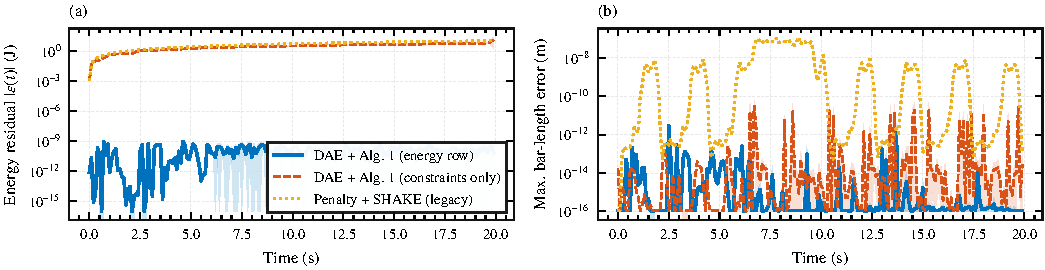
\includegraphics[width=\textwidth]{fig_physics_consistency.pdf}
\caption{Physical consistency under the SGT gait (Level 1, mean
$\pm1\sigma$ shaded). (a) Ledger residual $|\varepsilon(t)|$ after correction (held at the
solver tolerance by the energy row; it accumulates without it).
(b) Maximal bar-length error. Solid: DAE with energy row; dashed: DAE
with constraint rows only; dotted: legacy penalty+SHAKE core.}
\label{fig:physics}
\end{figure*}

\subsection{Nominal locomotion}
With identical actuator limits and all aids disabled, SGT advances
$\nSgtProgress$\,m in 20\,s (\nSgtSpeed\,$\pm$\,\nSgtSpeedStd\,m/s,
\nSgtSuccess\,\% success; Table~\ref{tab:nominal}, Fig.~\ref{fig:nominal}),
about \speedRatio\ times the speed of the support-face heuristic. The
LQR, iLQR and QP-MPC schedulers optimize a scalar effort over the same
support-face primitive and therefore inherit its limitation: none of
them leaves the launch pad (at most \baseBestProgress\,m), and their
cost of transport is an order of magnitude higher. This is a statement
about the primitive, which cannot shift the COM of the 5.8\,kg system
over an edge within a 0.15\,m stroke, rather than about the optimizers.
SGT plans in \nSgtSolveMs\,ms on average (worst \nSgtSolveMax\,ms) in
single-threaded JavaScript, well inside its 50\,ms control period. Its
main weakness is heading: the greedy per-cycle edge choice produces a
zig-zag track with a cross-track RMSE of \nSgtRmse\,m
(full ground tracks are in the released run files).


\begin{figure*}[t]
\centering
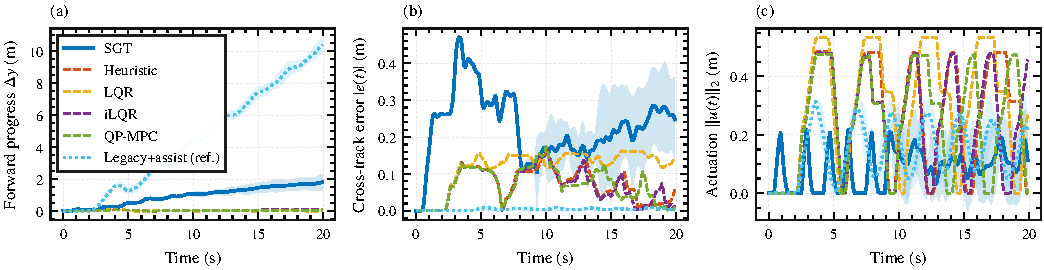
\includegraphics[width=\textwidth]{fig_nominal_locomotion.pdf}
\caption{Nominal cable-only locomotion (5 seeds, mean $\pm1\sigma$).
(a) Forward progress. (b) Cross-track error. (c) Actuation norm.
Solid: proposed; dashed: baselines; dotted: inadmissible reference.}
\label{fig:nominal}
\end{figure*}

\begin{figure}[t]
\centering
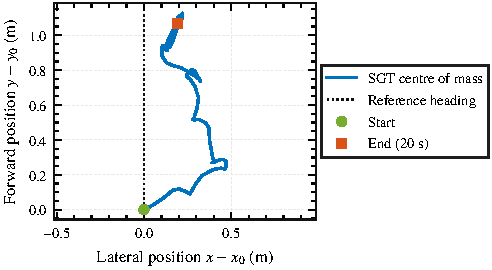
\includegraphics[width=\columnwidth]{fig_sgt_path.pdf}
\caption{Ground track of the COM under SGT (seed 1, 20\,s).}
\label{fig:path}
\end{figure}

\subsection{Robustness}
table~\ref{tab:stress} summarizes the stress
tests (3 seeds each). SGT keeps rolling after a 0.5\,m/s lateral impulse
(\sImpSpeed\,m/s) and under a 10\,N, 2\,s push (\sPushSpeed\,m/s), and
is insensitive to $-40\,\%$ friction (\sFricSpeed\,m/s) and $+30\,\%$
payload mass (\sMassSpeed\,m/s). Softer cables ($-20\,\%$) slow it to
\sStiffSpeed\,m/s because the same stroke produces smaller COM shifts,
and a 100\,ms actuation delay to \sDelaySpeed\,m/s
(\sDelaySuccess\,\% success). Measurement noise is the main weakness:
Gaussian noise reduces the speed to \sGaussSpeed\,m/s, while
heavy-tailed noise is damaging---Laplace noise to \sLapSpeed\,m/s
(\sLapSuccess\,\% success) and 2\,\% outliers to \sOutSpeed\,m/s. SGT uses
the measured node positions both to detect the support face and to
assemble $\vect K$, so a single corrupted node can trigger a wrong face
or edge; a robust state estimator in front of the planner is required
before hardware use.


\begin{figure}[t]
\centering
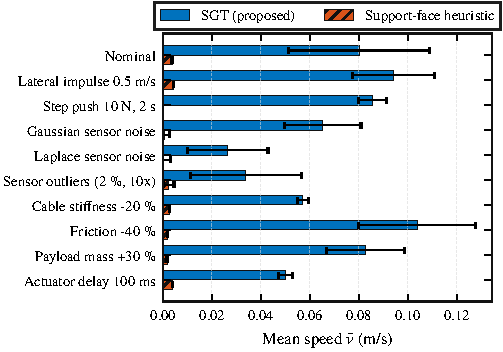
\includegraphics[width=\columnwidth]{fig_robustness.pdf}
\caption{Mean speed under disturbances, sensor noise, plant mismatch and
delay (3 seeds, error bars $\pm1\sigma$).}
\label{fig:robust}
\end{figure}

\subsection{Ablation and terrain}
table~\ref{tab:ablation} isolates the ingredients of SGT (3 seeds).
Removing the bars' geometric stiffness is the most harmful change:
speed drops from \aFullSpeed\ to \aNoGeoSpeed\,m/s, success to
\aNoGeoSuccess\,\% and the cost of transport nearly doubles
(\aNoGeoCot\ vs.\ \aFullCot), confirming that the softening of the
compressed bars is what the sensitivity has to capture. The other design
choices did not help in our tests: without payload actuation the speed
is essentially unchanged (\aNoPayloadSpeed\,m/s) at a lower cost of
transport (\aNoPayloadCot); restricting the command to the 8 most
sensitive cables keeps the speed (\aSparseSpeed\,m/s) and gives the
lowest cost of transport (\aSparseCot); and choosing the edge by
alignment with the travel direction instead of by reachable margin was
not worse (\aNoFeasSpeed\,$\pm$\,\aNoFeasSpeedStd\,m/s). With three
seeds these differences are within one standard deviation, so we report
the margin-based rule as specified before the experiments and leave the
sparse, payload-free variant as the more efficient configuration. Run
on the penalty+SHAKE core without aids, the same controller reaches only
\aLegacySpeed\,m/s: the projection that absorbs the cable work also
absorbs the deformation that SGT relies on. Results on rougher
terrain are in the Appendix (Table~\ref{tab:terrain}).


\begin{figure}[t]
\centering
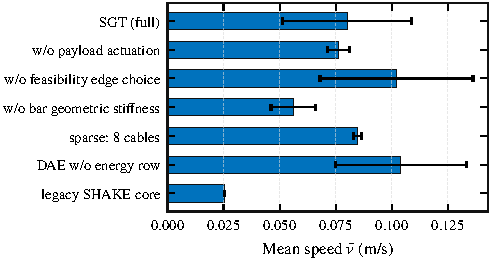
\includegraphics[width=\columnwidth]{fig_ablation.pdf}
\caption{Ablation of SGT components and of the physics core (3 seeds).}
\label{fig:ablation}
\end{figure}

% Auto-generated by tools/make_extension_tables.mjs -- do not edit by hand.
\begin{table}[t]
\centering
\caption{MPC + GPS on 4 held-out conditions (20\,s, mean\,$\pm$\,std).}
\label{tab:gps}
\setlength{\tabcolsep}{3.2pt}
\renewcommand{\arraystretch}{1.08}
\footnotesize
\begin{tabular}{@{}lcccc@{}}
\toprule
Controller & Progress\,$\uparrow$ & Tips\,$\uparrow$ & Aborts\,$\downarrow$ & $t_{\mathrm{ctrl}}$\,$\downarrow$ \\
 & {\scriptsize (m)} & & & {\scriptsize (ms)} \\
\midrule
SGT \eqref{eq:sgt} & 2.11\,{\scriptsize$\pm$0.34} & 11.0\,{\scriptsize$\pm$1.4} & \textbf{0.25}\,{\scriptsize$\pm$0.50} & \textbf{0.53}\,{\scriptsize$\pm$0.05} \\
MPC teacher \eqref{eq:teacher}, $\lambda=0$ & \textbf{2.27}\,{\scriptsize$\pm$0.32} & 10.8\,{\scriptsize$\pm$1.3} & \textbf{0.25}\,{\scriptsize$\pm$0.50} & 0.63\,{\scriptsize$\pm$0.04} \\
MPC + GPS policy $\pi_\theta$ & 1.89\,{\scriptsize$\pm$0.47} & \textbf{11.5}\,{\scriptsize$\pm$1.7} & 0.50\,{\scriptsize$\pm$0.58} & 0.73\,{\scriptsize$\pm$0.05} \\
\bottomrule
\end{tabular}
\par\vspace{3pt}\parbox{\columnwidth}{\scriptsize\raggedright Held out: unseen seeds, Levels 1 and 3, straight and $\pm6$\,m offset goals. Aborts: tip cycles ended by the shift or tip timeout.}
\end{table}

\begin{table*}[t]
\centering
\caption{Suspension-integrity filter on 10 paired conditions (20\,s, mean\,$\pm$\,std over conditions).}
\label{tab:shield}
\setlength{\tabcolsep}{4pt}
\renewcommand{\arraystretch}{1.08}
\footnotesize
\begin{tabular}{@{}lcccccc@{}}
\toprule
 & \multicolumn{3}{c}{SGT} & \multicolumn{3}{c}{MPC + GPS policy} \\
\cmidrule(lr){2-4}\cmidrule(l){5-7}
Metric & Filter off & Filter on & Wins & Filter off & Filter on & Wins \\
\midrule
\multicolumn{7}{@{}l}{\textit{Suspension}} \\
\quad Payload-cable slack time (\%)\,$\downarrow$ & 35.1\,{\scriptsize$\pm$2.9} & \textbf{2.7}\,{\scriptsize$\pm$0.6} & 10/10 & 33.6\,{\scriptsize$\pm$2.4} & \textbf{1.6}\,{\scriptsize$\pm$0.6} & 10/10 \\
\quad Mean payload-cable tension (N)\,$\uparrow$ & 6.2\,{\scriptsize$\pm$0.5} & \textbf{18.0}\,{\scriptsize$\pm$1.0} & 10/10 & 6.9\,{\scriptsize$\pm$0.6} & \textbf{17.5}\,{\scriptsize$\pm$0.8} & 10/10 \\
\quad Payload rattle, RMS (mm)\,$\downarrow$ & 18.6\,{\scriptsize$\pm$1.0} & \textbf{15.0}\,{\scriptsize$\pm$2.5} & 9/10 & \textbf{22.4}\,{\scriptsize$\pm$1.0} & 27.5\,{\scriptsize$\pm$4.6} & 3/10 \\
\addlinespace[2pt]
\multicolumn{7}{@{}l}{\textit{Locomotion}} \\
\quad Progress $\Delta y$ (m)\,$\uparrow$ & 1.49\,{\scriptsize$\pm$0.39} & \textbf{2.20}\,{\scriptsize$\pm$0.64} & 8/10 & \textbf{1.32}\,{\scriptsize$\pm$0.64} & 1.29\,{\scriptsize$\pm$0.54} & 4/10 \\
\quad Aborted tip cycles\,$\downarrow$ & 1.1\,{\scriptsize$\pm$1.1} & \textbf{0.0}\,{\scriptsize$\pm$0.0} & 6/10 & \textbf{1.5}\,{\scriptsize$\pm$1.4} & 1.7\,{\scriptsize$\pm$1.4} & 3/10 \\
\addlinespace[2pt]
\multicolumn{7}{@{}l}{\textit{Peak loads (not certified, Remark~2)}} \\
\quad Payload accel., 99th pct (g)\,$\downarrow$ & \textbf{2.50}\,{\scriptsize$\pm$1.08} & 3.18\,{\scriptsize$\pm$1.70} & 4/10 & 2.04\,{\scriptsize$\pm$1.12} & \textbf{1.71}\,{\scriptsize$\pm$0.66} & 5/10 \\
\quad Min payload--rod clearance (m)\,$\uparrow$ & \textbf{0.102}\,{\scriptsize$\pm$0.018} & 0.090\,{\scriptsize$\pm$0.035} & 5/10 & \textbf{0.105}\,{\scriptsize$\pm$0.014} & 0.101\,{\scriptsize$\pm$0.033} & 4/10 \\
\quad Max outer-cable tension (N)\,$\downarrow$ & \textbf{137}\,{\scriptsize$\pm$81} & 179\,{\scriptsize$\pm$79} & 3/10 & 122\,{\scriptsize$\pm$65} & \textbf{105}\,{\scriptsize$\pm$52} & 7/10 \\
\addlinespace[2pt]
\multicolumn{7}{@{}l}{\textit{Cost}} \\
\quad Controller time (ms)\,$\downarrow$ & \textbf{0.64}\,{\scriptsize$\pm$0.11} & 3.60\,{\scriptsize$\pm$0.21} & -- & \textbf{0.79}\,{\scriptsize$\pm$0.12} & 3.64\,{\scriptsize$\pm$0.23} & -- \\
\bottomrule
\end{tabular}
\par\vspace{3pt}\parbox{\textwidth}{\scriptsize\raggedright Conditions: three seeds on Level~1, two on Level~3, push, impulse, payload $+30\,\%$, 100\,ms actuation delay and cable stiffness $-20\,\%$. Wins: paired conditions in which the filter improved the metric. Bold: better mean. Metrics exclude the first second (initial settling).}
\end{table*}


\subsection{MPC + GPS}
On the held-out conditions the learned policy advances
\gpsPolicyProgress\,m in 20\,s, \gpsRatio\,\% of SGT
(\gpsSgtProgress\,m) and \gpsTeacherRatio\,\% of the teacher
(\gpsTeacherProgress\,m), with \gpsPolicyAborts\ aborted cycles per run
(Table~\ref{tab:gps}). It exceeds SGT in one condition
(\gpsBestPolicy\,m vs.\ \gpsBestSgt\,m). The unregularized teacher is
itself slightly faster than SGT, which we attribute to its rate-aware
smoothing. The policy is not cheaper per tick in our implementation
(\gpsPolicyMs\ vs.\ \gpsSgtMs\,ms): for 13 nodes the KKT solve is already
inexpensive, so the value of the policy lies in replacing the model
evaluation by a learned map, not in speed.

\subsection{Suspension integrity}
With the filter the payload cables are slack \shSlackOnSgt\,\% of the
time under SGT (\shSlackOffSgt\,\% without) and \shSlackOnGps\,\% under
the policy (\shSlackOffGps\,\%), in all \shConditions\ conditions
(Table~\ref{tab:shield}); the mean payload-cable tension rises from
\shTensionOffSgt\ to \shTensionOnSgt\,N. For SGT the taut suspension
also makes tipping more effective: progress increases from
\shProgOffSgt\ to \shProgOnSgt\,m ($+\shProgGainSgt\,\%$, better in
\shProgBetterSgt\ of \shConditions\ conditions) and aborted cycles fall
from \shAbortOffSgt\ to \shAbortOnSgt. For the policy, whose progress is
unchanged (\shProgOffGps\ vs.\ \shProgOnGps\,m), the filter restores the
suspension at no cost in progress. The filter does not reduce peak
loads: in \shClearViol\ of \shFilteredRuns\ filtered runs the payload
came closer than 0.08\,m to a rod (minimum \shClearMin\,m), in
\shOuterViol\ runs an outer cable exceeded 150\,N, and the
99th-percentile payload acceleration of SGT increased. These are the
inertial events outside the quasi-static prediction
(Section~\ref{sec:shield}). The filter adds \shMs\,ms per control step.

% ---------------------------------------------------------------------
\section{Limitations}\label{sec:limits}
All results are in simulation. The contact parameters ($k$, $\alpha$,
$\mu$) and cable stiffnesses were not identified on hardware, so absolute
speeds will not transfer directly; what the ledger provides is a bound
on the energy contributed by the integrator, projections and aids, not
a validation of the model against reality. The time-step study uses a
single seed. SGT is sensitive to heavy-tailed measurement noise
(Section~\ref{sec:results}) and needs a robust estimator before
hardware use. SGT is quasi-static: it ignores inertia during the tip and
re-plans only at 20\,Hz, which limits speed to the order of
\SI{0.1}{m/s}. Edge selection is greedy per cycle, which causes the
zig-zag ground track and cross-track error visible in
Fig.~\ref{fig:path}; a heading-aware selection over several faces is a
natural extension. The baselines inherit a reduced-order model and the
support-face primitive from the original code base; stronger
whole-body optimal controllers may close part of the gap, and the
released protocol is intended to make such comparisons easy.

The MPC + GPS policy imitates a teacher built on the same quasi-static
model, so it inherits its limitations and is evaluated on
\gpsEvalConditions\ held-out conditions only; it still needs one KKT
solve per tip cycle for edge selection and is not faster than SGT. The
suspension-integrity filter certifies its constraints only for the
quasi-static prediction: payload clearance and cable loads during
tumbling and impacts are not guaranteed, which requires a second-order
barrier on the DAE dynamics. Finally, the modelled shell is a regular
icosahedron (offset ratio $d/h=1/\varphi$); a form-finding analysis
with the TsgFEM equilibrium matrix \cite{ma2022tsgfem} shows that this
shape admits no self-stress state, whereas the expanded octahedron
($d/h=0.5$) admits one. The modelled rest geometry is therefore not a
prestressed equilibrium, and the shell deforms away from it as soon as
the simulation starts; part of the sag reported in
Section~\ref{sec:shield} may originate here, and repeating the study on
the form-found shape is future work.

\section{Conclusion}
We showed how to make tensegrity-rover simulation \emph{auditable}: a
non-minimal Lagrangian DAE with exact multipliers, a minimum-norm
constraint-and-energy corrector, passive contact with a potential and a
work ledger that measures the unexplained energy of every step before
it is corrected. The ledger shows that this drift is first-order
discretization error in the proposed core, and it exposes the
kilojoule-scale projection exchange and the non-physical aids of a
conventional penalty+projection engine. On this basis, the
sensitivity-gradient tipping gait achieves cable-only rolling of a
six-bar rover with a heavy payload where reduced-order effort schedulers
over a fixed primitive do not; the bars' geometric stiffness is the
ingredient of the sensitivity that matters most. The same sensitivity
model serves as the teacher of an MPC-guided policy search (MPC + GPS)
whose learned per-cable policy reaches \gpsRatio\,\% of SGT's progress,
and as the prediction model of a suspension-integrity filter that keeps
the payload cables taut and, by preserving the tipping shift, makes SGT
\shProgGainSgt\,\% faster. Code, run files and the scripts that
generate every table and figure are released with the paper.

\section*{Reproducibility}
\texttt{npm run experiments} executes the full protocol
(114 runs, resumable), \texttt{npm run paper:data} regenerates
\texttt{tables.tex}, \texttt{numbers.tex} and all figures, and
\texttt{node tools/drift\_check.mjs} repeats the time-step study; the same
protocol runs in the browser (\emph{Comparative benchmark} panel).
\texttt{node tools/train\_guided\_policy.mjs} trains and evaluates the
MPC + GPS policy, \texttt{node tools/run\_shield\_study.mjs} and
\texttt{node tools/measure\_sag.mjs} produce the filter study, and
\texttt{node tools/make\_extension\_tables.mjs} regenerates
Tables~\ref{tab:gps} and~\ref{tab:shield} and their numbers.

\bibliographystyle{IEEEtran}
\bibliography{references}

\end{document}
